% Section 3: Useful context on real data
% Required packages: \usepackage{amsmath,booktabs,graphicx}
% Upload this file together with the vector figures in figures/.
% The GiftEval reference is defined in references.bib.

\section{Useful context on real data}
\label{sec:real-context}

We first ask whether context-length selection is relevant on real forecasting
tasks, independently of whether it can be predicted.  Specifically, how much
history is useful, how much does that quantity vary across tasks, and what
accuracy--compute opportunity does this variation create?  We answer these
questions using post-hoc window ablations on GiftEval
\cite{aksu2024gifteval}.  All choices in this section use realized test errors
and are therefore diagnostic oracles, not deployable selectors.  Learned
selection is introduced only in the following section.

\subsection{Window-ablation protocol}
\label{sec:real-protocol}

We evaluate the 97 dataset--forecast-term cells in the official GiftEval
cohort, comprising 371{,}330 forecast instances.  For every time-series
foundation model (TSFM), cell $c$, and forecast instance $i$, we rerun the same
forecast over every feasible context length in the predefined grid
$\mathcal{G}_c$.  A requested grid length is capped by the history available to
that instance; grid values that are not supported by the model or data are
excluded.  Forecast quality is measured with the leaderboard-faithful
\texttt{mase\_gluonts\_real} implementation.  Following the leaderboard, we
normalize the MASE in each cell by the corresponding Seasonal-Naive value and
aggregate cells with a geometric mean.  For a policy $\pi$,
\begin{equation}
    \operatorname{nMASE}(\pi)
    = \exp\!\left[
        \frac{1}{|\mathcal{C}|}
        \sum_{c\in\mathcal{C}}
        \log\!\left(
            \frac{\operatorname{MASE}_c(\pi)}
                 {\operatorname{MASE}^{\mathrm{SN}}_c}
        \right)
      \right],
    \qquad |\mathcal{C}|=97.
    \label{eq:normalized-mase}
\end{equation}
This cell-balanced aggregation prevents large datasets from dominating the
benchmark score.

We distinguish four reference policies.  \emph{Native/full} supplies each
forecast with its maximum available context.  A \emph{global fixed window}
uses one requested length for every cell, capped only when less history is
available.  The \emph{cell-shared oracle} selects one hindsight-optimal action
per dataset--term cell,
\begin{equation}
    L_c^{\star}
    \in \arg\min_{L\in\mathcal{G}_c\cup\{\mathrm{native}\}}
        \operatorname{MASE}_c(L),
    \label{eq:cell-oracle}
\end{equation}
and then shares this action across every instance in that cell.  Finally, the
\emph{instance oracle} chooses a hindsight-optimal length separately for each
forecast instance.  The cell-shared oracle is a dataset-level diagnostic that
preserves a realistic action granularity, whereas the instance oracle is an
unattainable upper bound that quantifies within-cell heterogeneity.  Neither
oracle has access to information available at deployment time: both use the
realized forecast outcomes.

\subsection{Context sensitivity is real and heterogeneous}
\label{sec:real-heterogeneity}

Figure~\ref{fig:real-context-curves} illustrates four qualitatively different
behaviors among cells with native histories of approximately 8,000 steps.
On KDDCup2018-H at the long forecast term, error generally decreases as more
history is provided and the oracle lies near the longest available context.
Solar-H at the medium term instead favors a short window.  JenaWeather-10T at the long term has an
interior optimum: both aggressive truncation and the longest contexts are
inferior.  BitbrainsRnD-5T exhibits a broad optimum over several intermediate
windows, making the precise choice comparatively less important.
Thus, the effect is not a uniform preference for either short or long context;
even within one model, real cells can exhibit opposite or non-monotonic
responses.

\begin{figure*}[t]
    \centering
    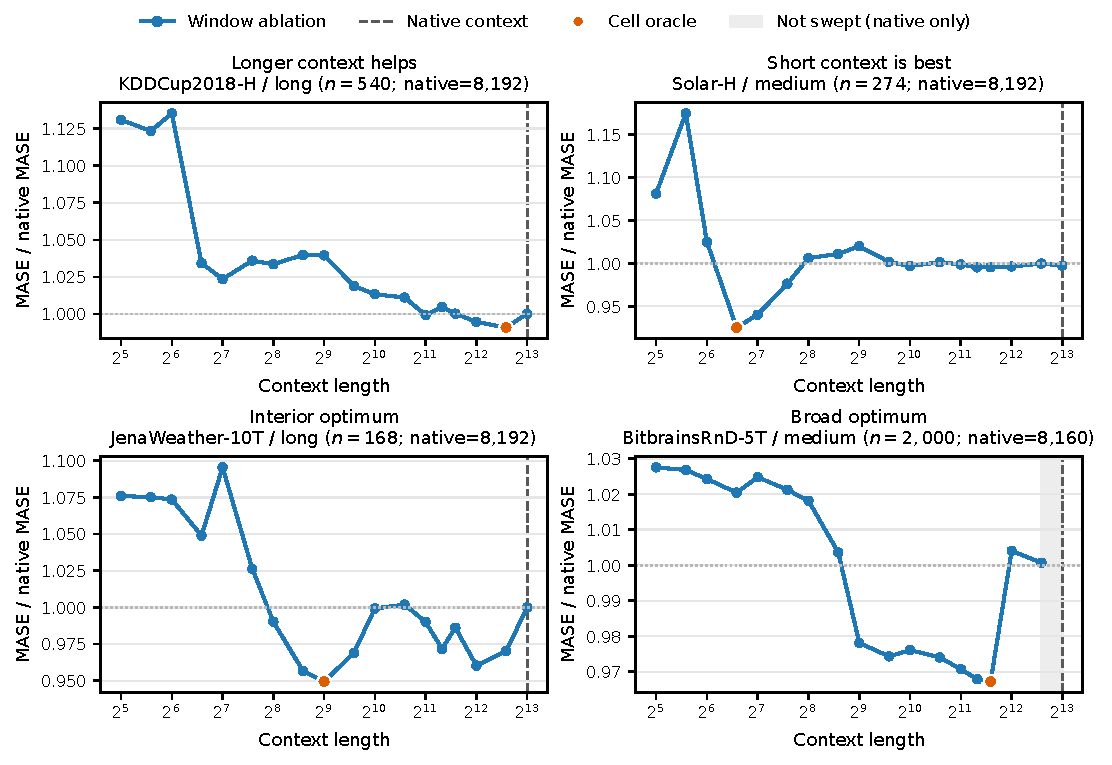
\includegraphics[width=\textwidth]{figures/fig3_context_case_studies.pdf}
    \caption{Representative context-window ablations for Chronos2-Small on
    four real GiftEval cells with native histories of 8,160--8,192 steps.
    Each curve reports cell MASE relative to the native-context MASE; values
    below one improve on native.  The vertical
    dashed line denotes the native context, the filled orange marker denotes
    the hindsight cell oracle, and light shading marks the interval not swept
    by shortened-window ablations (where only the native baseline is available).
    Cases were selected to be well populated and to
    show distinct, non-pathological behaviors rather than the largest observed
    gains.}
    \label{fig:real-context-curves}
\end{figure*}

The same heterogeneity persists across the complete 97-cell cohort.  The cell
oracle uses less than native context in 72 of 97 cells (74.2\%).  Among these shortened cells, the
median selected length is only 31.25\% of native context; across all cells, the
median ratio is 50\%.  Shortening is also often an accuracy intervention rather
than merely a computational approximation: 69 cells improve by more than
0.1\%, and 49 improve by more than 1\%.  At the same time, several cells remain
at native context, and the selected ratios span more than two orders of
magnitude.  Useful context is therefore neither globally fixed nor
consistently equal to the maximum available history.

\subsection{The accuracy--compute opportunity}
\label{sec:real-pareto}

We next measure how much of this heterogeneity can be converted into a joint
accuracy--compute gain.  At each point on the frontier, the oracle still chooses
only one action per cell.  We enumerate the exact supported frontier induced by
a non-negative global FLOPs penalty,
\begin{equation}
    \min_{\{L_c\}}
    \frac{1}{|\mathcal{C}|}
    \sum_{c\in\mathcal{C}}
       \log\!\left(
          \frac{\operatorname{MASE}_c(L_c)}
               {\operatorname{MASE}^{\mathrm{SN}}_c}
       \right)
    + \lambda
      \frac{\sum_{c\in\mathcal{C}}\operatorname{FLOPs}_c(L_c)}
           {\sum_{c\in\mathcal{C}}\operatorname{FLOPs}_c(\mathrm{native})},
    \qquad \lambda\geq 0.
    \label{eq:oracle-pareto}
\end{equation}
The main analysis balances compute equally across the 97 cells, matching the
cell-balanced accuracy aggregation in Equation~\ref{eq:normalized-mase}.
Workload-weighted compute, which multiplies each cell by its number of forecast
instances, answers a separate serving-cost question and is reported in the
supplement.

Figure~\ref{fig:real-oracle-pareto} shows a broad favorable region.  Native
context obtains normalized MASE 0.7267.  The unconstrained minimum-MASE oracle
improves this to 0.7047, a 3.03\% relative reduction, while simultaneously
saving 52.9\% of theoretical FLOPs.  Allowing normalized MASE to remain within
0.5\% and 1\% of the oracle minimum increases savings to 73.8\% and 78.2\%,
respectively.  The most compute-efficient supported point that is no worse than
native reaches normalized MASE 0.7247 while saving 85.0\% of FLOPs.  Beyond
this region the curve steepens sharply: the minimum-compute endpoint saves
94.3\%, but its normalized MASE degrades to 1.0460.  Hence the practical oracle
knee lies around 74--85\% FLOPs saved, well before the minimum-compute extreme.

\begin{figure*}[t]
    \centering
    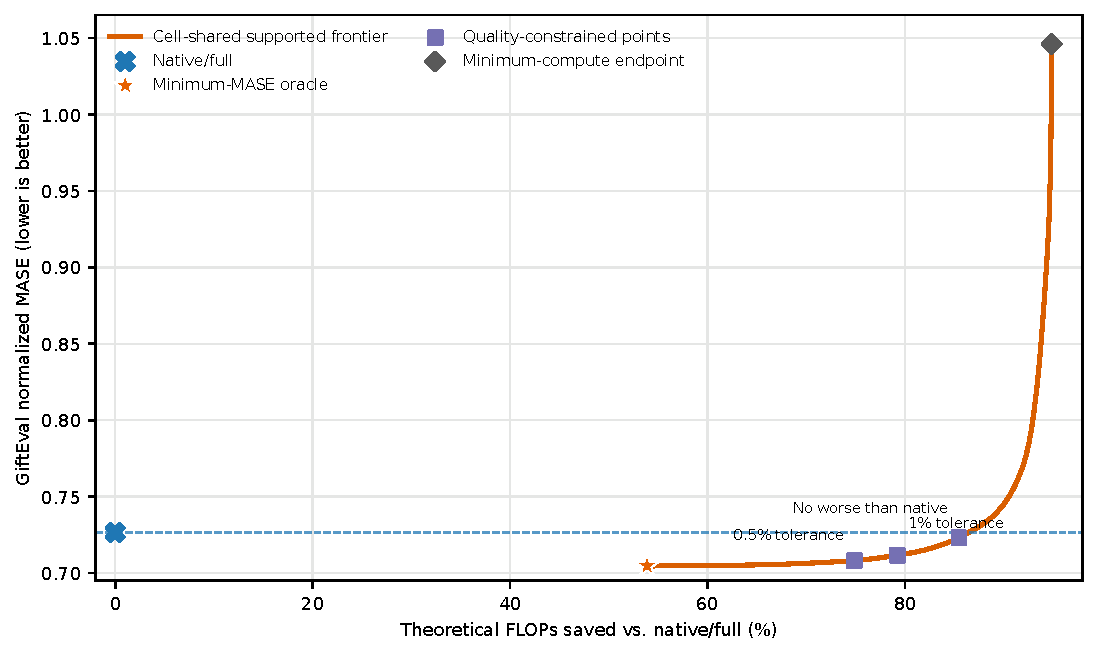
\includegraphics[width=0.94\textwidth]{figures/fig5_cell_oracle_pareto.pdf}
    \caption{Cell-shared oracle accuracy--compute frontier for
    Chronos2-Small on GiftEval.  The oracle chooses one context action per
    dataset--term cell.  Compute is the cell-balanced sum of theoretical FLOPs,
    and quality is the 97-cell normalized MASE in
    Equation~\ref{eq:normalized-mase}.  Markers identify native/full context,
    the minimum-MASE oracle, accuracy-constrained operating points, and the
    minimum-compute supported endpoint.  Learned selectors are deliberately
    excluded because this figure measures diagnostic headroom.}
    \label{fig:real-oracle-pareto}
\end{figure*}

\subsection{Model-level scope}
\label{sec:real-model-scope}

We repeat the identical window grid, leaderboard-faithful metric, and corrected
model-specific FLOPs accounting for 11 TSFMs.  Every model admits a cell-shared
oracle that is both more accurate and cheaper than native context
(Figure~\ref{fig:multimodel-oracle-forest}).  At the minimum-MASE oracle, the
relative accuracy improvement ranges from 1.00\% to 4.30\%, while theoretical
FLOPs savings range from 5.79\% to 52.92\%.  Moving along each supported
frontier while requiring accuracy no worse than native increases the attainable
savings to 12.72--89.40\% (Table~\ref{tab:real-oracle-models}).

\begin{figure*}[t]
    \centering
    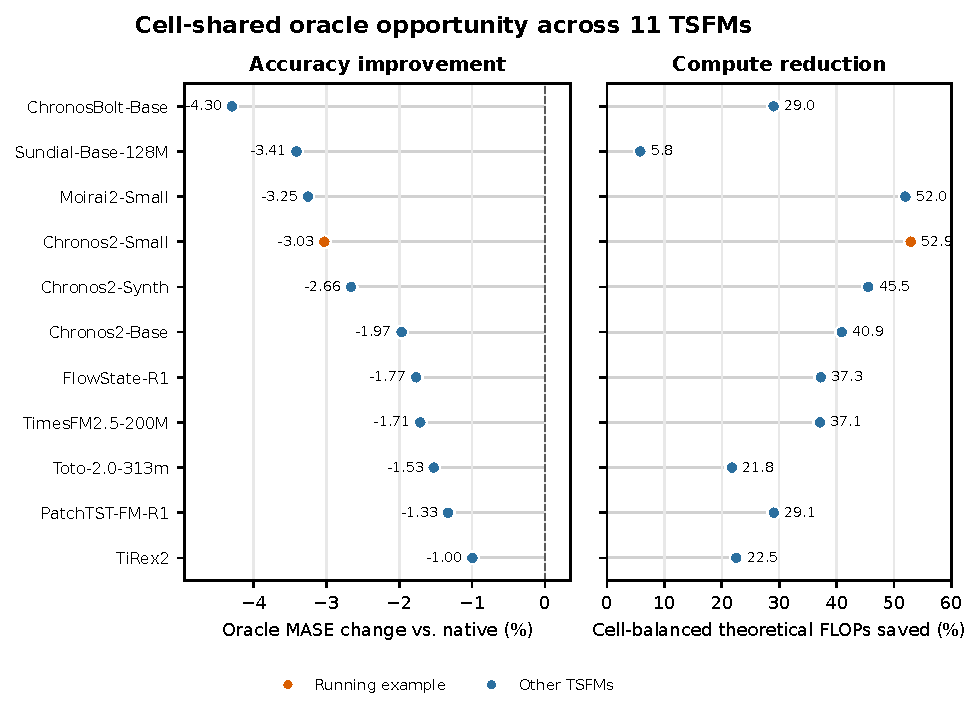
\includegraphics[width=0.94\textwidth]
        {figures/fig6_multimodel_oracle_forest.pdf}
    \caption{Cell-shared oracle opportunity across 11 TSFMs on the 97-cell
    GiftEval cohort.  The left panel reports the relative change in normalized
    MASE from native context to the minimum-MASE cell oracle (more negative is
    better); the right panel reports the simultaneous reduction in
    cell-balanced theoretical FLOPs.  Chronos2-Small is highlighted in orange.}
    \label{fig:multimodel-oracle-forest}
\end{figure*}

The superposed frontiers in Figure~\ref{fig:multimodel-pareto-overlay} show that
the favorable region is not limited to a single operating point or model.  We
divide each model's normalized MASE by its native value so that all native
baselines coincide at one.  The displayed range is capped at $1.10\times$
native MASE and confirms the expected steep quality loss as compute is reduced.
The location of the knee remains
model dependent, motivating a learned selector rather than one universal
context-reduction rule.

\begin{figure*}[t]
    \centering
    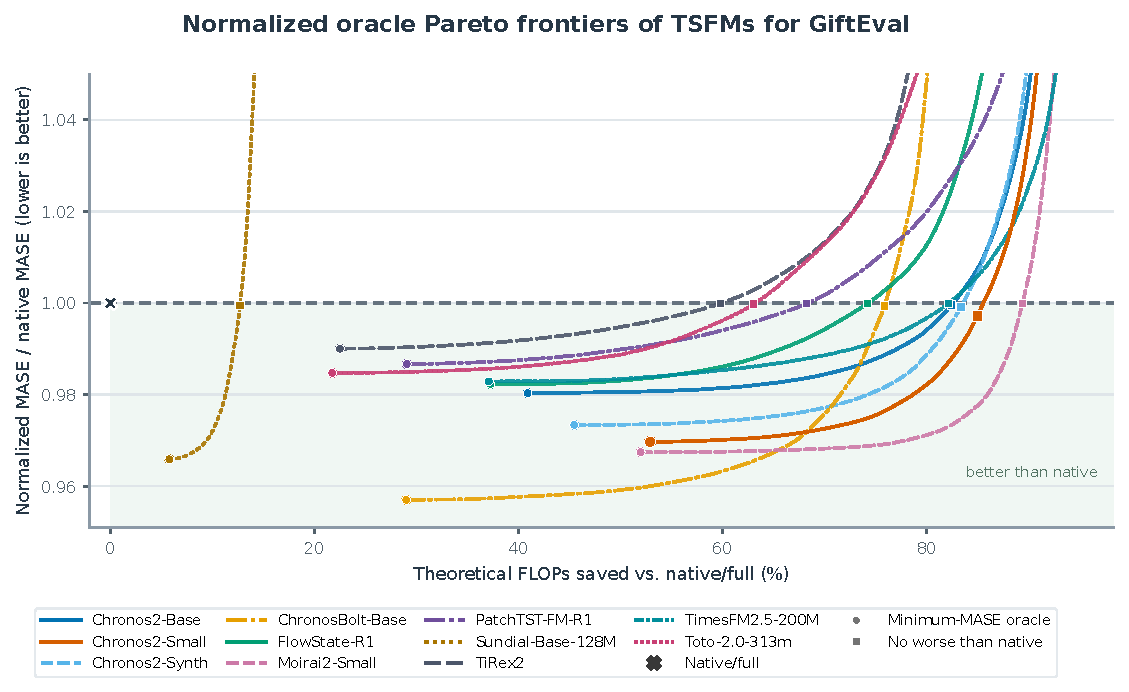
\includegraphics[width=0.98\textwidth]
        {figures/fig7_multimodel_pareto_overlay.pdf}
    \caption{Superposed cell-shared supported Pareto frontiers for 11 TSFMs.
    Normalized MASE is divided by each model's native-context value; the dashed
    horizontal reference therefore denotes native accuracy.  The vertical
    range extends to $1.10\times$ native MASE; supported points above that
    limit are clipped.
    Circles mark the minimum-MASE oracles and
    squares mark the greatest supported FLOPs reduction that remains no worse
    than native.  Chronos2-Small is highlighted in orange.}
    \label{fig:multimodel-pareto-overlay}
\end{figure*}

\begin{table*}[t]
    \centering
    \footnotesize
    \setlength{\tabcolsep}{5pt}
    \caption{Cell-shared oracle and supported-frontier results.  ``Oracle
    save'' is the theoretical FLOPs reduction at the minimum-MASE oracle;
    ``no-worse save'' is the largest supported reduction whose normalized MASE
    does not exceed the native value.  ``Pareto pts.'' counts distinct
    supported-frontier policies selected for at least one value of $\lambda$ in
    Equation~\ref{eq:oracle-pareto}; it is not a count of datasets or cells.}
    \label{tab:real-oracle-models}
    \begin{tabular}{lrrrrrr}
        \toprule
        Model & Native & Oracle & $\Delta$ MASE & Oracle save & No-worse save & Pareto pts. \\
        \midrule
        Chronos2-Base       & 0.7047 & 0.6909 & $-1.97\%$ & 40.91\% & 82.47\% & 487 \\
        Chronos2-Small      & 0.7267 & 0.7047 & $-3.03\%$ & 52.92\% & 84.99\% & 476 \\
        Chronos2-Synth      & 0.7352 & 0.7157 & $-2.66\%$ & 45.49\% & 83.38\% & 474 \\
        ChronosBolt-Base    & 0.8096 & 0.7748 & $-4.30\%$ & 29.02\% & 75.87\% & 402 \\
        FlowState-R1        & 0.7090 & 0.6965 & $-1.77\%$ & 37.26\% & 74.24\% & 467 \\
        Moirai2-Small       & 0.7378 & 0.7138 & $-3.25\%$ & 51.98\% & 89.40\% & 483 \\
        PatchTST-FM-R1      & 0.7045 & 0.6952 & $-1.33\%$ & 29.06\% & 68.25\% & 541 \\
        Sundial-Base-128M   & 0.7507 & 0.7251 & $-3.41\%$ &  5.79\% & 12.72\% & 474 \\
        TiRex2              & 0.6967 & 0.6897 & $-1.00\%$ & 22.52\% & 59.82\% & 541 \\
        TimesFM2.5-200M     & 0.7050 & 0.6930 & $-1.71\%$ & 37.10\% & 82.19\% & 515 \\
        Toto-2.0-313m       & 0.7040 & 0.6932 & $-1.53\%$ & 21.77\% & 63.07\% & 499 \\
        \bottomrule
    \end{tabular}
\end{table*}

\subsection{From diagnostic opportunity to prediction}
\label{sec:real-bridge}

The real-data ablations reveal substantial opportunity, but do not explain why
forecast quality saturates or deteriorates with additional history.  Before
introducing a deployable selector, the next section asks whether distant
observations are genuinely unused, whether models can extend their reach when
long-range information becomes necessary, and whether apparent context effects
are partly induced by preprocessing.  The learned context-response predictor
is introduced in the section that follows.
